\section{Design and Implementation}
\label{sec:imp}

This section details the design and implementation of our proof of concept tool
--- \venera --- as it stands so far. It is comprised of two parts: and an
Android instrumentation application and a Jenkins plugin.
We describe the tool from the bottom up;
\autoref{sec:sec:android_instrumentation} covers the Android instrumentation and
\autoref{sec:sec:jenkins_plugin} describes the structure of the Jenkins plugin.

\subsection{\venera}
\label{sec:sec:android_instrumentation}

The \venera repository\cite{heisentestInstrumentation} is made up of a number of
modules. Figure \ref{fig:repo_structure} shows an overview of the structure and
key submodules.

\begin{figure}[h]
    \dirtree{%
    .1 venera.
    .2 dex-generator\DTcomment{An Android application from which ASMDEX visitor
    code is generated}.
    .2 dexifier\DTcomment{A Java command line tool that generates ASMDEX visitor
    code given a {\tt .apk}}.
    .2 skeleton-android-app\DTcomment{A basic Android application, with
    Espresso\cite{espresso}-based tests}.
    .2 venera-instrumentation\DTcomment{A Java command line tool responsible
    for the actual instrumentation}.
    .2 venera-sdk\DTcomment{A standalone Java library that defines the {\tt
    @Venera} annotation}.
    }
\caption{\venera module structure}
\label{fig:repo_structure}
\end{figure}

The main tool --- found under the {\tt venera-instrumentation} directory --- is
operated from the command line. It takes a number of required arguments. If any
of the arguments are missing, a usage message is printed and the program exits.

\begin{itemize}
    \item {\tt applicationApk} --- The fully qualified path to the Application
    APK to be instrumented.
    \item {\tt testApk} --- The fully qualified path to the Application Test APK
    to be instrumented.
    \item {\tt baseTestCaseInfo} --- A comma seperated list of tuples consisting
    of: the full name of a base test case class, followed by the short names of
    its set up and tear down methods. Must have at least one element.
\end{itemize}

An example usage, run from the directory containing both of the APKs to be
instrumented, would look something like:

\texttt{
  venera --applicationApk=android-app-debug.apk\\
  --testApk=android-app-debug-test.apk\\
  --baseTestCaseInfo=com.example.BaseTestCase,setUp,tearDown
}

\subsubsection{The Android Platform}

It is necessary to give an overview of the Android platform in order to
understand how \venera works.

In a standard Java application, code is compiled into {\tt .class} files and
packaged as a {\tt .jar} --- an archive containing compiled {\tt .class} files,
resources, a manifest and certificates. A Java compiler will generate one class
file per type (including inner and anonymous) present in the source program. At
runtime, the bytecode in these classes is executed by the Java Virtual Machine.

Similarly, Android applications are written in Java and compiled to bytecode.
However, the target Virtual Machine --- Dalvik --- is register-based, so the
bytecode is transformed after compilation. The {\tt dx} tool is used to convert
multiple {\tt .class} files to a single {\tt .dex} file\footnote{Note that an
Android application can be defined over multiple {\tt dex} files, but this is
not the norm and requires custom class loading.} and packaged as an {\tt .apk}.
Like the standard {\tt .jar} file, an Android {\tt .apk} is simply an archive
containing the compiled assets for an Android application.

For the purposes of the instrumentation, many of the included files can be
ignored. Figure \ref{fig:android_apk} shows the contents of an {\tt APK}
relevant to our tool. For an application with device-based tests (\ie, the
applications we target), an application test {\tt APK} will also be generated
when the tests are run. The test archive contains the compiled test source code
and is executed when the tests are run.

\begin{figure}[h]
\dirtree{%
.1 application.apk.
.2 META-INF\DTcomment{Directory containing certificates}.
.2 AndroidManifest.xml\DTcomment{Basic info --- version, name, etc.}.
.2 classes.dex\DTcomment{Dalvik bytecode (register-based format)}.
}
\caption{}
\label{fig:android_apk}
\end{figure}

\venera broadly follows the same set of steps for both the application and
test {\tt APK}s. Figure \ref{fig:instrumenting_apk} shows each of the steps in
the order they occur. First, the application {\tt .apk} is extracted. Then, the
{\tt classes.dex} file is parsed two times: the first pass inspects the
bytecode, the second injects our instrumentation. Finally, the {\tt APK} is
re-packaged, the tests are run, and the results are collected. Afterward, the
Jenkins plugin takes over.

\begin{figure}[h]
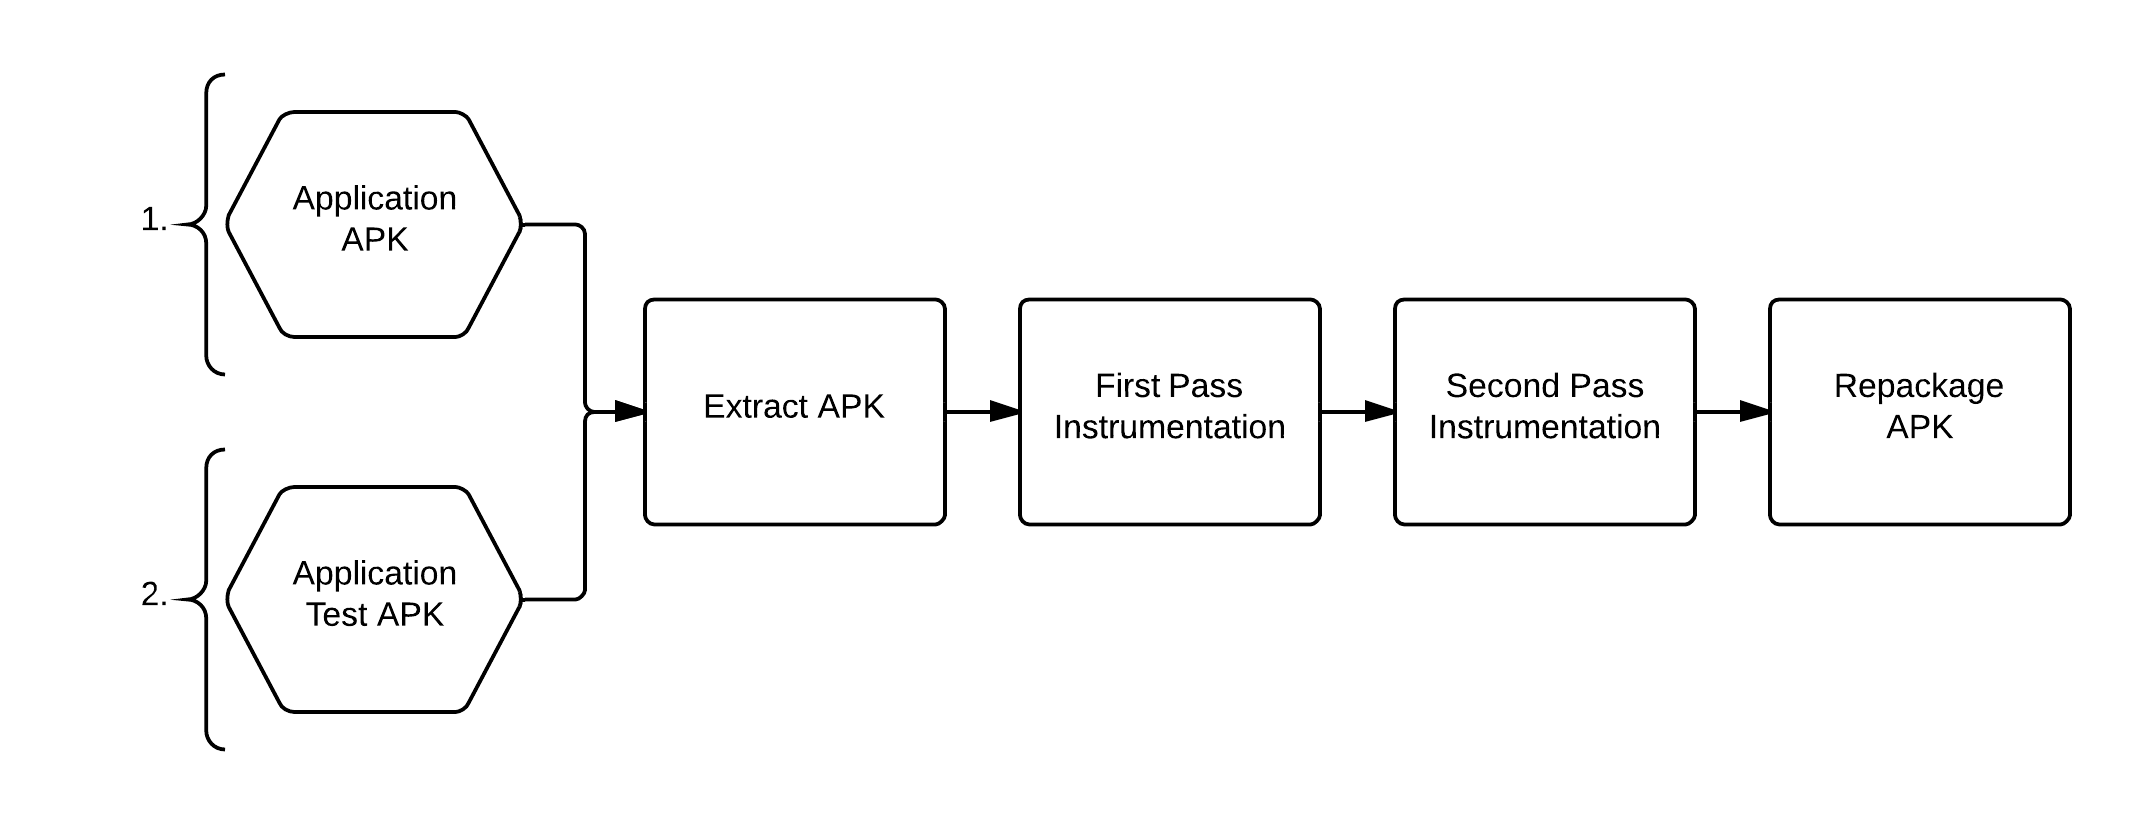
\includegraphics[width=\linewidth]{Images/instrumenting_apk}
\caption{}
\label{fig:instrumenting_apk}
\end{figure}

\subsubsection{Extraction}

\subsubsection{First Pass}

The first time, we build up a list of {\tt InstrumentationPoint} objects. These
correspond to the instrumentation points defined in
\autoref{sec:sec:instrumentation_points}. The proof of concept supports method
entry instrumentation points, and has basic infrastructure for branch points,
but no working support. At the moment, our implementation is not adaptive ---
instrumentation points are added unconditionally provided they match a certain
signature (\eg, method entry). Each {\tt InstrumentationPoint} object has an
associated {\tt InstrumentationPolicy}. The tool assumes an {\tt
InstrumentationPolicy} of {\tt Complex} for now, unless a {\tt @Venera}
annotation is found with a different policy. \autoref{sec:sec:venera_sdk}
defines the {\tt @Venera} annotation and its customizable parameters. Note
that in the future, instrumentation points and the like will be stored along
with the test run results by the Jenkins plugin. Then, the results will be given
to this tool again, so that it can decide which instrumentation policies to
apply to each instrumentation point (\eg, an instrumentation point with a
previous {\tt InstrumentationPolicy} of {\tt InstrumentationPolicy.COMPLEX}
could be assigned a new policy of {\tt InstrumentationPolicy.NONE} if the site
has not been helpful in determining a failure-predicting predicate and should
not be monitored this time around).

\subsubsection{Second Pass}

Instrumentation bytecode is injected during the second pass. With a list of
instrumentation points defined, we visit the bytecode again, this time inserting
probes based on the {\tt InstrumentationPolicy} each time we encounter bytecode
that matches a known {\tt InstrumentationPoint}. As might be expected, a policy
of {\tt COMPLEX} tells us to inject a complex probe, {\tt SIMPLE} a simple
(counter-based) probe and {\tt NONE} nothing at all.

The user must provide at least one base test class and the names of its
equivalent JUnit's {\tt SetUp} and {\tt TearDown} methods. These are methods
that are called respectively at the beginning and end of each individual test
run. We inject code to initialize and clean up our logging system at these
points. Upon {\tt SetUp}, we create a file matching the test name to store
runtime data.

\subsubsection{The Event System}

Complex probes serialize Java objects to JSON with google-gson. Primitives are
boxed to their object representations.

\subsubsection{Injecting Instrumentation}

This section details the steps we take to insert probe at an instance method
entry and presents the results of both a complex and a simple probe in practice.

A Dalvik bytecode method consists of the definition and associated data. Most of
this data is of no consequence to our instrumentation, but we have to pay
attention to the registers.

Each method specifies the number of registers it requires. Arguments of a method
take the final registers, with the final argument taking the final register
position. Instance methods have a reference to their live object passed as the
first argument; the formal arguments (if any) take up the next registers in
order.

For the Java methods:

\begin{lstlisting}[mathescape, numberblanklines=false]
private String anExampleMethod(String firstArg, int secondArg) {
    return appendIntToString(firstArg, secondArg);
} (*@\SuppressNumber@*)
$\vdots$ (*@\ReactivateNumber@*)
private static String appendIntToString(String baseString, int number) {
    return baseString + number;
}
\end{lstlisting}

The corresponding Dalvik bytecode would be generated for {\tt anExampleMethod}\footnote{Note that this listing omits irrelevant
sections of bytecode. The full listing can be found in
\autoref{sec:sec:full_dalvik_bytecode_example}.}:

\begin{lstlisting}[mathescape,numberblanklines=false]
#1              : (in Lcom/example/MainActivity;)
  name          : 'anExampleMethod'
  type          : '(Ljava/lang/String;I)Ljava/lang/String;'
  access        : 0x0002 (PRIVATE) (*@\SuppressNumber@*)
$\vdots$ (*@\ReactivateNumber@*)
  registers     : 4
  ins           : 3
  outs          : 2 (*@\SuppressNumber@*)
$\vdots$ (*@\ReactivateNumber@*)
024570:                  |[024570] com.example.MainActivity.anExampleMethod:(Ljava/lang/String;I)Ljava/lang/String; (*@\label{method_body_definition}@*)
024580: 7120 8503 3200   |0000: invoke-static {v2, v3}, Lcom/example/MainActivity;.appendIntToString:(Ljava/lang/String;I)Ljava/lang/String; // method@0385
024586: 0c00             |0003: move-result-object v0
024588: 1100             |0004: return-object v0 (*@\label{method_body_end_definition}@*) (*@\SuppressNumber@*)
$\vdots$ (*@\ReactivateNumber@*)
      locals    :
        0x0000 - 0x0005 reg=1 this Lcom/example/MainActivity;
        0x0000 - 0x0005 reg=2 firstArg Ljava/lang/String;
        0x0000 - 0x0005 reg=3 secondArg I
\end{lstlisting}

Lines \ref{method_body_definition}-\ref{method_body_end_definition} define the
method body. In this case, the method body simply returns void since it is empty
in the original Java source. The full set of bytecode operations and symbols are
defined at \cite{dalvikBytecode}. From here on we will focus on the
registers, method body and locals of the bytecode, omitting extraneous
information as we see fit.

\begin{lstlisting}[label=instrumented_example]
    #1              : (in Lcom/heisentest/skeletonandroidapp/test/unit/MainActivityTest;)
      name          : 'anExampleMethod'
      type          : '(Ljava/lang/String;I)Ljava/lang/String;'
      access        : 0x0002 (PRIVATE)
      registers     : 12
      ins           : 3
      outs          : 7 (*@\SuppressNumber@*)
$\vdots$ (*@\ReactivateNumber@*)
      locals        :
        0x0000 - 0x0030 reg=9 this Lcom/heisentest/skeletonandroidapp/test/unit/MainActivityTest;
        0x0000 - 0x0030 reg=10 firstArg Ljava/lang/String;
        0x0000 - 0x0030 reg=11 secondArg I
\end{lstlisting}

\autoref{instrumented_example} shows the bytecode after a Complex Instance
Method Entry probe has been added. It is clear after inspecting the full listing
included in \autoref{sec:sec:full_dalvik_instrumented_bytecode_example} that our
Complex Instance Method Entry probe is doing a lot of work. Indeed, the probe
must {\lq}box{\rq} any primitive arguments (\ie, convert them into a Java
object), set up an {\tt Object} array and more. This is why the Complex probes
carry such a high overhead as show in \autoref{sec:sec:probe_cost}.

The reference to the instance object ({\tt this}) is shifted up to
register 9 by our instrumentation, along with all of the following method
parameters. Our instrumentation does its work using registers 0 to 8, and simply
moves the argument parameters back to their original positions after the work is
done. Our class --- {\tt RegisterAllocatingMethodVisitor} --- can be subclassed
by any instrumenting method visitor to implement this functionality. This is a
useful piece of functionality, since otherwise register manipulation is tedious
and prone to error.

Our instrumentation process is built around ASMDEX's architecture. Unfamiliarity
with the library meant that comprimises were made in the name of time. The most
significant of these is the register shifting present in all of our
instrumentation. We override ASMDEX's {\tt visitMaxs} method to request
additional registers with which to do our work (\ie, to log our events). Since
this occurs \textit{after} the original method bytecode is generated, we must
shift the argument parameters back to their original positions at the end of our
instrumentation. Future versions of \venera could be made more efficient by
eliminating this register shifting.

\subsubsection{\venera SDK}
\label{sec:sec:venera_sdk}

A small project under the {\tt venera-sdk} directory defines the main event
logging system ({\tt HeisentestJsonLogger}) and event beans (subclassed from
{\tt LogEvent}). The \venera SDK also defines the annotation {\tt @Venera} and its
associated parameter of type {\tt InstrumentationPolicy}. During the
instrumentation phase, if a method is found with this annotation, its policy
is applied unconditionally. This could be useful for developers during
debugging --- it allows them to prevent sites from being instrumented or to
specifify an exact instrumentation type from the available policies:
\begin{itemize}
  \item {\tt NONE} --- Disallows any instrumentation from being injected into
  the method. When a test is annotated with this parameter, the logging system
  itself will not be initialized for that test.
  \item {\tt SIMPLE} --- Disallows complex probes from being injected into the
  containing method.
  \item {\tt COMPLEX} --- (Default), allows all probes to be placed
  in the containing method if needs be.
\end{itemize}

During setup, if the currently executing method has a {\tt @Venera} annotation
attached, we look at its policy before running the logging set up. If the
annotation has {\tt InstrumentationPolicy.NONE}, we simply run the test as normal.

This means that within a class with multiple tests, we can disable
instrumentation on any subset of the tests if the developer so desires.

It is important to note that while the {\tt @Venera} annotation with an
instrumentation policy of {\tt NONE} prevents the method itself from being
instrumented (and in the case of a test, also prevents the logging system from
being initialized), other methods will \textit{still} potentially be
instrumented. So a test with the annotation and policy that initializes an
Android {\tt Activity} and performs a sequence of actions will still have a
performance penalty if called methods happen to be instrumented.

\subsection{Logging to JSON}

Our logging system is event based. Each probe calls an log method with some
parameters. The logging method creates an event bean in memory. The bean is put
into a blocking queue and held until it can be written to the {\tt .json} output
file. We define an abstract {\tt LogEvent} bean with common values (System Time,
Thread ID, EventName etc.) and implement subclasses for specific events.

The background thread in charge of logging the events to disk serialises the
data to {\tt JSON} before writing it to a file.

\autoref{lst:json_log} shows an example output from one of the the fully
instrumented (\ie, {\tt COMPLEX}) test runs performed in
\autoref{sec:sec:probe_cost}. It tells us the method
\textit{anInstrumentedEmptyMethod} was entered at system millisecond time
\textit{1398719422295} by the thread with id \textit{51708}. Since it was a
{\tt COMPLEX} probe, we also get the name and value of any actual arguments
(\lineref{line:begin_params} to \lineref{line:end_params}).

\begin{lstlisting}[label=lst:json_log]
[
  {
    "eventType": "Complex Instance Method Entry",
    "threadId": 51708,
    "time": 1398719422295,
    "class": "com.heisentest.skeletonandroidapp.test.acceptance.ProbeTest",
    "method": "anInstrumentedEmptyMethod",
    "parameters": [(*@\label{line:begin_params}@*)
      {
        "unusedParameter": "0"
      }
    ](*@\label{line:end_params}@*)
  }
]
\end{lstlisting}

\subsubsection{Storing the Results}

With the tests running on the Android device or emulator, we must somehow
retrieve the {\tt JSON} logs either during the test run or afterward.
Transferring logs during the test run is unreliable. If we were to send our JSON
to {\tt logcat} with a special tag and monitor it on the build agent, we could
{\lq}miss{\rq} messages due to log flooding. Consider a heavily instrumented
application capable of logging a huge number of events in a short period of time
--- if data is written to the device's log buffer faster than {\tt logcat} can
read out of it, messages will be dropped. Instead, we log the {\tt JSON} to
files on the device's storage and retrieve it when the test suite has finished
running.

Copying the {\tt .json} log files back to the computer running the
instrumentation from the device with Gradle is a little tricky. Android provides
private storage for each installed application. It is possible, with root user
permissions, to access files in this space to manipulate them. However, as soon
as the tests finish executing, the Android Gradle plugin runs a private task
that uninstalls the application. When an application is removed, all of its
private data is deleted. Because the uninstall task is private, it is not
possible to hook in and run a simple shell script to retrieve the logs before
they are deleted.

We devised a workaround; Android has guaranteed {\lq}public{\rq} storage that is
not removed when an application is uninstalled. Its location is not fixed and is
likely to differ per-device and operating system version. So, we take care to
inform the build agent of the exact location of the device's public storage each
test run before copying the files.

When the tests finish running, we log a message with a special tag to {\tt
logcat} specifying the full path to the results directory on the device. Then, a
Gradle task grabs the {\tt logcat} logs, searches for the message and parses it
to get the location. Then, the task uses {\tt adb pull} and {\tt adb rm} to grab
and finally delete the files from the device. The previous issue of log flooding
can still be a problem here. If our special log message is lost in the noise of
an extreme number of log messages (i.e., deleted before we can grab it), the
build could fail. This is robust enough for a proof of concept.

\subsubsection{Soot}
\label{sec:sec:sec:soot}

We looked into Soot for its ability to generate control flow graphs (CFGs). When
searching for failure-predicting predicates, we will favour locations further
down the CFG when placing probes (new or moved). It is possible to generate the
CFG for a method using ASMDEX alone, although it is a slightly more tricky task,
and one that we have not tackled so far.

In the end, although Soot appeared to be a nice tool to work with, we scrapped
it for a few reasons. Firstly, the representation used by Soot is fairly
incompatible with that of ASMDEX. Even if we could determine the CFG for a
method using Soot, we'd have to somehow map the locations to our ASMDEX
instrumentation sites --- a non-trivial task. Finally, the overhead of starting
up Soot and loading an APK is significant. On an
Intel\textsuperscript{\textregistered} Core\textsuperscript{\texttrademark}
i7-3610QM CPU @ 2.30GHz, the time to load the application and test APKs was
10.76 seconds. With a total instrumentation time of 19.09 seconds, Soot takes up
56\% of the total instrumentation time (and that is \textit{without} generating
the CFGs for any methods). In fact, with Soot removed entirely, the same
instrumentation run took just 3.294 seconds --- 17\% of the previous total run
time.

We could have used Soot to convert Dalvik bytecode into standard Java {\tt
.class} files using Dexpler \cite{bartel:soap2012} and instrumented from then
on. This would have eliminated any incompatability concerns. However, the {\tt
dex} code output by Dexpler is often invalid, as is evident from the bug reports
and ongoing discussion at GitHub. Perhaps in the future, Soot will be a more
viable option. Certainly the features it boasts are attractive for our project.


\subsection{\jenkinsPlugin}
\label{sec:sec:jenkins_plugin}

In a typical software development project, continuous integration systems are
set up at the beginning. Developers write code and commit to source control. A
server running a Continuous Integration tool will detect the change and assign
one of a number of build agents (other servers with the capability to build the
project(s) - virtual or otherwise) an attached job.

For a typical job, the chosen build agent pulls down the latest changes,
compiles the code and runs the tests and any related tasks. At the end, any
build artifacts (distributable packages, test results, etc.) are uploaded to the
Continuous Integration server, freeing the agent to once again build the next
job in the queue. Note that in reality, a job can comprise of any number of
runnable steps --- from executing a shell script to hitting an external server.

It is obvious that, if we are to develop a tool to assist developers with \flaky
tests, we should run as part of a modular continuous integration system.

\subsubsection{A Choice of Continuous Integration Tools}

Jenkins \cite{Jenkins} is a popular open source continuous integration tool.
Like others of its kind, it maintains a history of build results and their
associated artifacts. A wealth of plugins provide support for testing frameworks
such as JUnit --- displaying individual test outcomes, stack traces and
assertions in a simple interface.

Although there are many open source alternatives which we could support (\eg,
Hudson, from which the Jenkins project derives), many of these have
significantly smaller user bases and commit activity.

Although the tool will be developed initially for Jenkins, it is essential to
structure the plugin such that it can easily be migrated to other Continuous
Integration systems. At all stages of design, this must be kept in mind.


\subsubsection{Architecture}

The Jenkins plugin manages the storage of the test results and associated
artifacts in a HSQL database. After a test run completes, we can gather the test
run artifacts (JUnit results, \venera {\tt JSON} log files \etc) and store them
in a persistent database. As it stands, the plugin does not feed any historical
information back to \venera. Alongside displaying information to the developers,
this will be its eventual role.
